\chapter{Data Analysis and Fundamental Machine Learning Techniques – (Units 1 and 2)}

\section{Overview of Allotted Topics}
\textbf{Unit 1, Exploratory Data Analysis (EDA)}, is the systematic examination of data before modelling: auditing
quality, cleaning, summarising distributions, measuring relationships and turning patterns into insights. It fits the
problem because the two allotted market datasets (Google Play Store \cite{playstore} and Video Game Sales \cite{vgsales}) contain no prediction target.
The goal is understanding: which apps and games succeed, and why. The key tools are robust summary statistics (median,
quantiles), rank correlation (Spearman's $\rho$, which is suited to the heavily skewed install and sales counts), and
log-scaled visualisation.

\textbf{Unit 2, Supervised learning}, learns a mapping $f:\mathbf{x}\mapsto y$ from labelled examples.
\begin{itemize}
\item \textbf{Regression} ($y\in\mathbb{R}$) is applied to the Combined Cycle Power Plant (CCPP) data \cite{tufekci}, predicting
net hourly electrical output from four ambient sensors.
\item \textbf{Classification} ($y\in\{0,1\}$) is applied to the Bank Marketing data \cite{moro}, predicting whether a client will
subscribe to a term deposit before being called.
\end{itemize}
Both datasets are tabular with well-defined targets, which makes them ideal for comparing linear models, instance-based
methods, kernel methods and tree ensembles under one evaluation protocol.

\section{Dataset Description}
\begin{table}[H]
\centering
\caption{Datasets used in Units 1 and 2}
\label{tab:ds12}
\renewcommand{\arraystretch}{1.25}
\begin{tabularx}{\linewidth}{@{}>{\raggedright\arraybackslash}p{2.6cm} >{\raggedright\arraybackslash}X c >{\raggedright\arraybackslash}p{3.3cm}@{}}
\toprule
\textbf{Dataset} & \textbf{Source} & \textbf{Rows $\times$ cols} & \textbf{Target} \\
\midrule
Google Play Store Apps & Kaggle, \texttt{lava18/google-play-store-apps} (2018 scrape) & 10,841 $\times$ 13 & none (EDA) \\
Video Game Sales & Kaggle, \texttt{gregorut/videogamesales} (VGChartz, 2016) & 16,598 $\times$ 11 & none (EDA) \\
Combined Cycle Power Plant & UCI ML Repository \#294 & 9,568 $\times$ 5 & PE, energy output (MW) \\
Bank Marketing (additional-full) & UCI ML Repository \#222 & 41,188 $\times$ 21 & y, subscribed (yes/no) \\
\bottomrule
\end{tabularx}
\end{table}
\begin{itemize}
\item \textbf{Play Store:} category, rating, reviews, size, installs, type, price, content rating, genres and update date.
Numbers are stored as text (``19M'', ``10,000+'', ``\$4.99''). There are 483 exact duplicates, a corrupted row, and 1,474
missing ratings.
\item \textbf{Video Game Sales:} platform, year, genre, publisher, and sales in millions for North America, Europe,
Japan, other regions and globally. 271 games have no year and 58 have no publisher.
\item \textbf{CCPP:} 9,568 hourly readings (2006–2011) of ambient temperature (AT, °C), exhaust vacuum (V, cm Hg),
ambient pressure (AP, mbar) and relative humidity (RH, \%), with no missing values.
\item \textbf{Bank Marketing:} 20 attributes covering the client, the campaign and the macro-economy. Only 11.3\% of
clients subscribe, so the classes are imbalanced. ``Unknown'' is used as a missing-value placeholder (e.g. 8,597 times in
\texttt{default}).
\end{itemize}
\textbf{Limitations:} the market datasets are snapshots (2016 and 2018). The video-game data counts only boxed retail
sales. The bank campaign spans the 2008–2010 financial crisis, so its macro-economic effects may not transfer to other
periods.

\section{Data Preprocessing}
\begin{itemize}
\item \textbf{Play Store:} dropped the corrupted row (columns shifted, Rating = 19) and the duplicates, keeping one row
per app (the most recent scrape): 10,841 $\rightarrow$ 9,659 apps. Converted text to numbers: size to MB (1,695 values of
``Varies with device'' set to missing), installs to integers, price to float. Engineered days-since-update and
$\log_{10}$ installs and reviews. Missing ratings (15.1\%) were \emph{not} imputed, because 92\% of them belong to apps
with $\le$1,000 installs: the missingness is informative.
\item \textbf{Video games:} dropped the 271 games with no year and restricted the data to $\le$2016 (later years are
incomplete): 16,323 games.
\item \textbf{CCPP:} removed 41 duplicate rows (9,527 remain), used an 80/20 split (7,621/1,906), and standardised features
inside a \texttt{Pipeline} so that the scaler is fitted on training folds only.
\item \textbf{Bank Marketing:} removed 12 duplicates. Dropped \texttt{duration} because it is \emph{target leakage}: the
call length is known only after the call has ended. Converted \texttt{pdays}=999 into a binary
\texttt{prev\_contacted} flag. Applied one-hot encoding (10 categorical features) and standardisation (9 numeric
features) in a \texttt{ColumnTransformer}, with a stratified 80/20 split (32,940/8,236).
\end{itemize}
\begin{pycode}
pre = ColumnTransformer([("num", StandardScaler(), num_cols),
                         ("cat", OneHotEncoder(handle_unknown="ignore"), cat_cols)])
X = df.drop(columns=["y", "target", "duration", "pdays"])      # leakage removed
X_train, X_test, y_train, y_test = train_test_split(X, y, test_size=0.2, stratify=y, random_state=42)
\end{pycode}

\section{Exploratory Data Analysis (EDA)}
\begin{figure}[H]
\centering
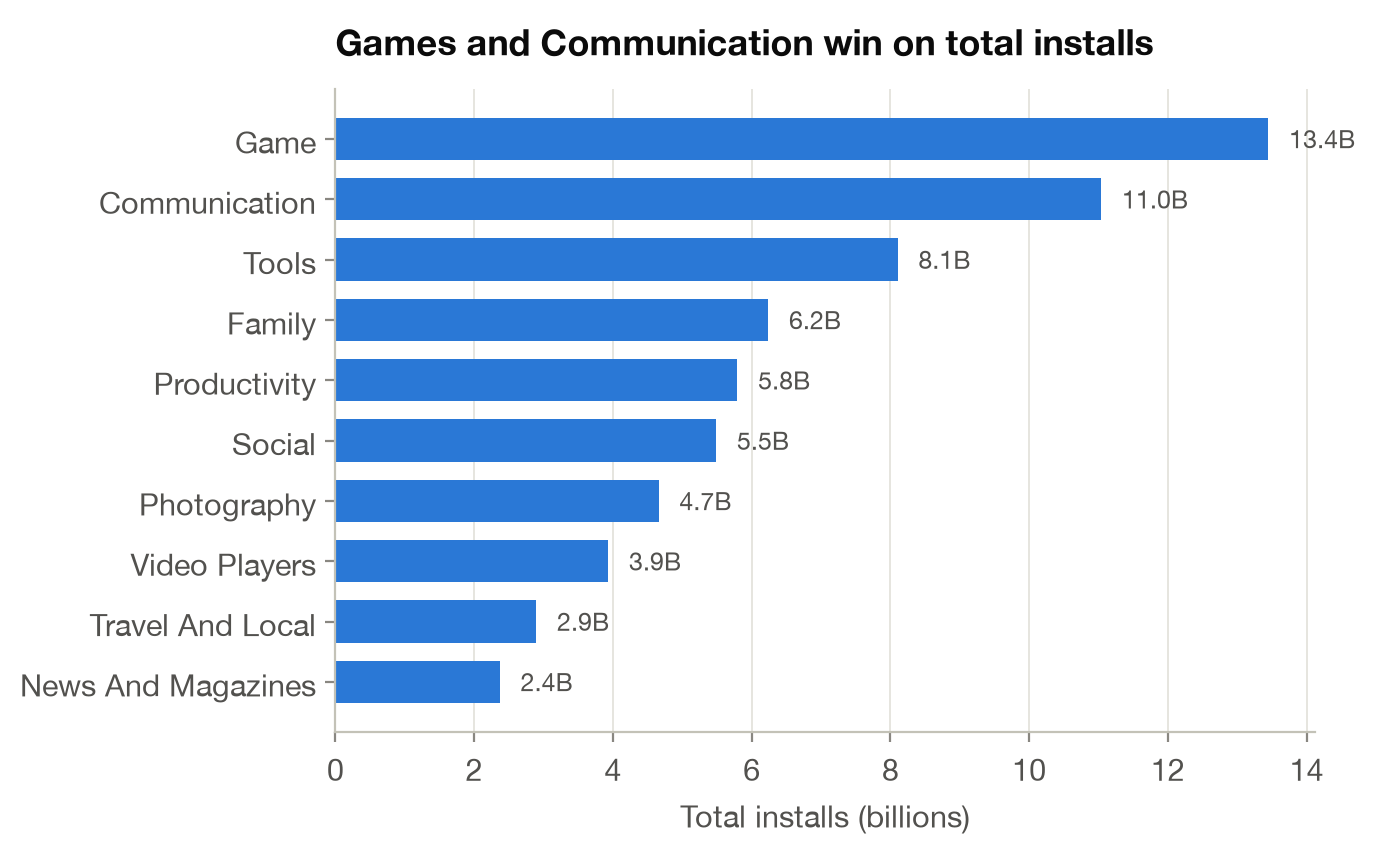
\includegraphics[width=0.49\linewidth]{ps_installs_by_category.png}\hfill
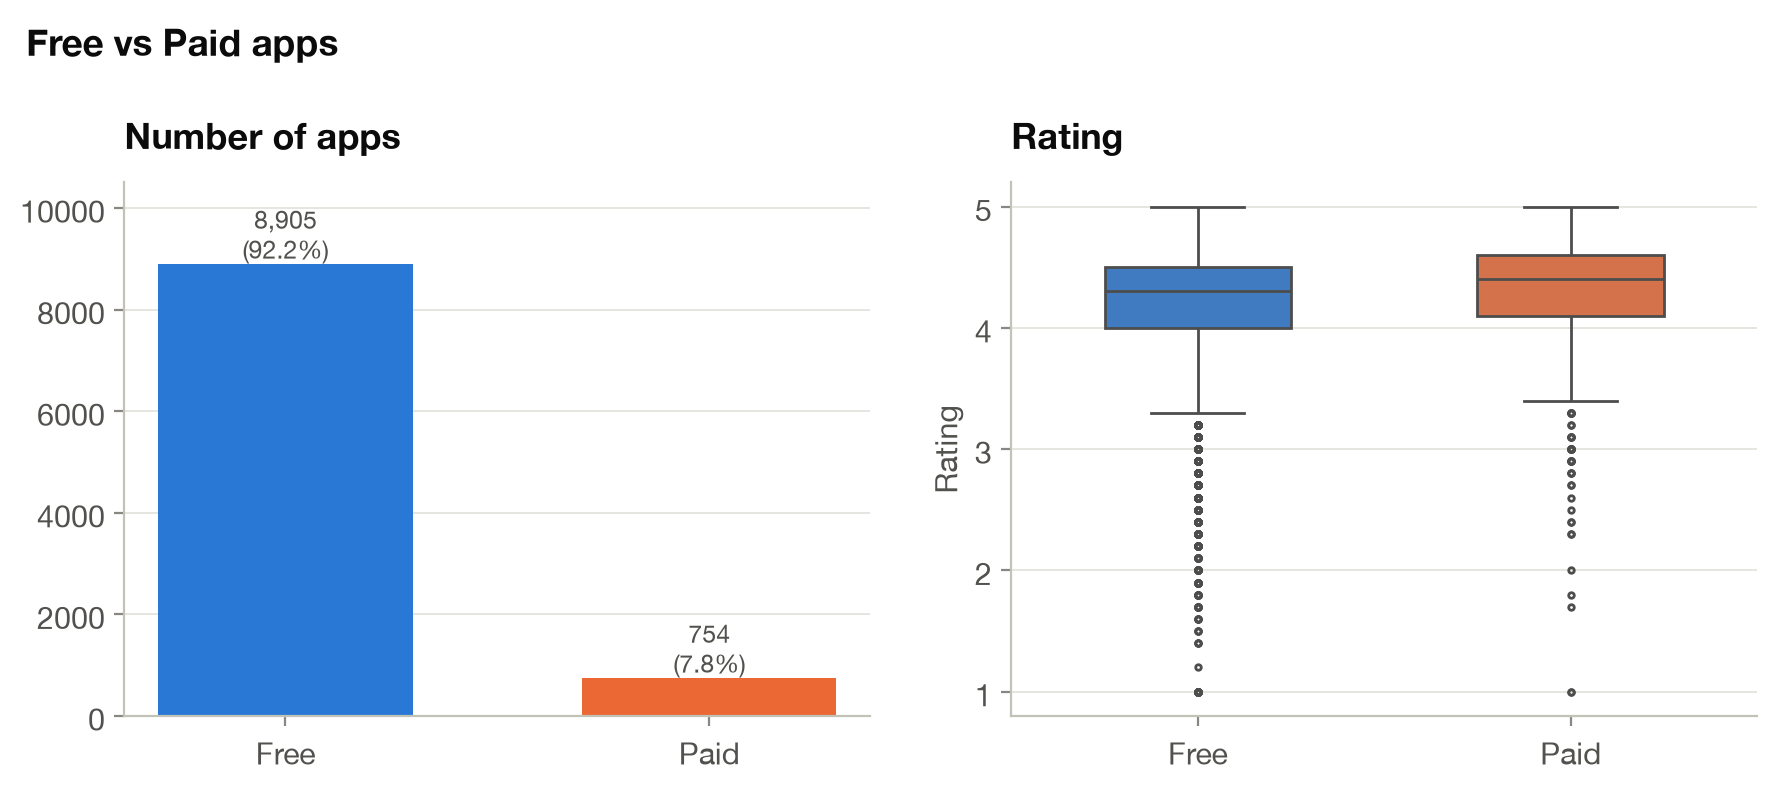
\includegraphics[width=0.49\linewidth]{ps_free_vs_paid.png}
\caption{Play Store: total installs by category (left) and free vs paid apps (right)}
\label{fig:ps}
\end{figure}
\textbf{Interpretation (Figure~\ref{fig:ps}).} Supply is not the same as demand. Family has the most apps (1,878), but
Game (13.4 billion installs) and Communication (11.0 billion) collect the most installs. Free apps are 92.2\% of the
store, and the median free app has 100,000 installs against 1,000 for a paid app. Paid apps are rated slightly higher
(4.26 vs 4.17). Ratings are inflated (median 4.3; 77\% of rated apps score $\ge$4.0). Reviews track installs almost
perfectly (Spearman $\rho=0.97$). Apps updated within the last month average 4.27 stars, against 4.05 for apps left
untouched for two years.

\begin{figure}[H]
\centering
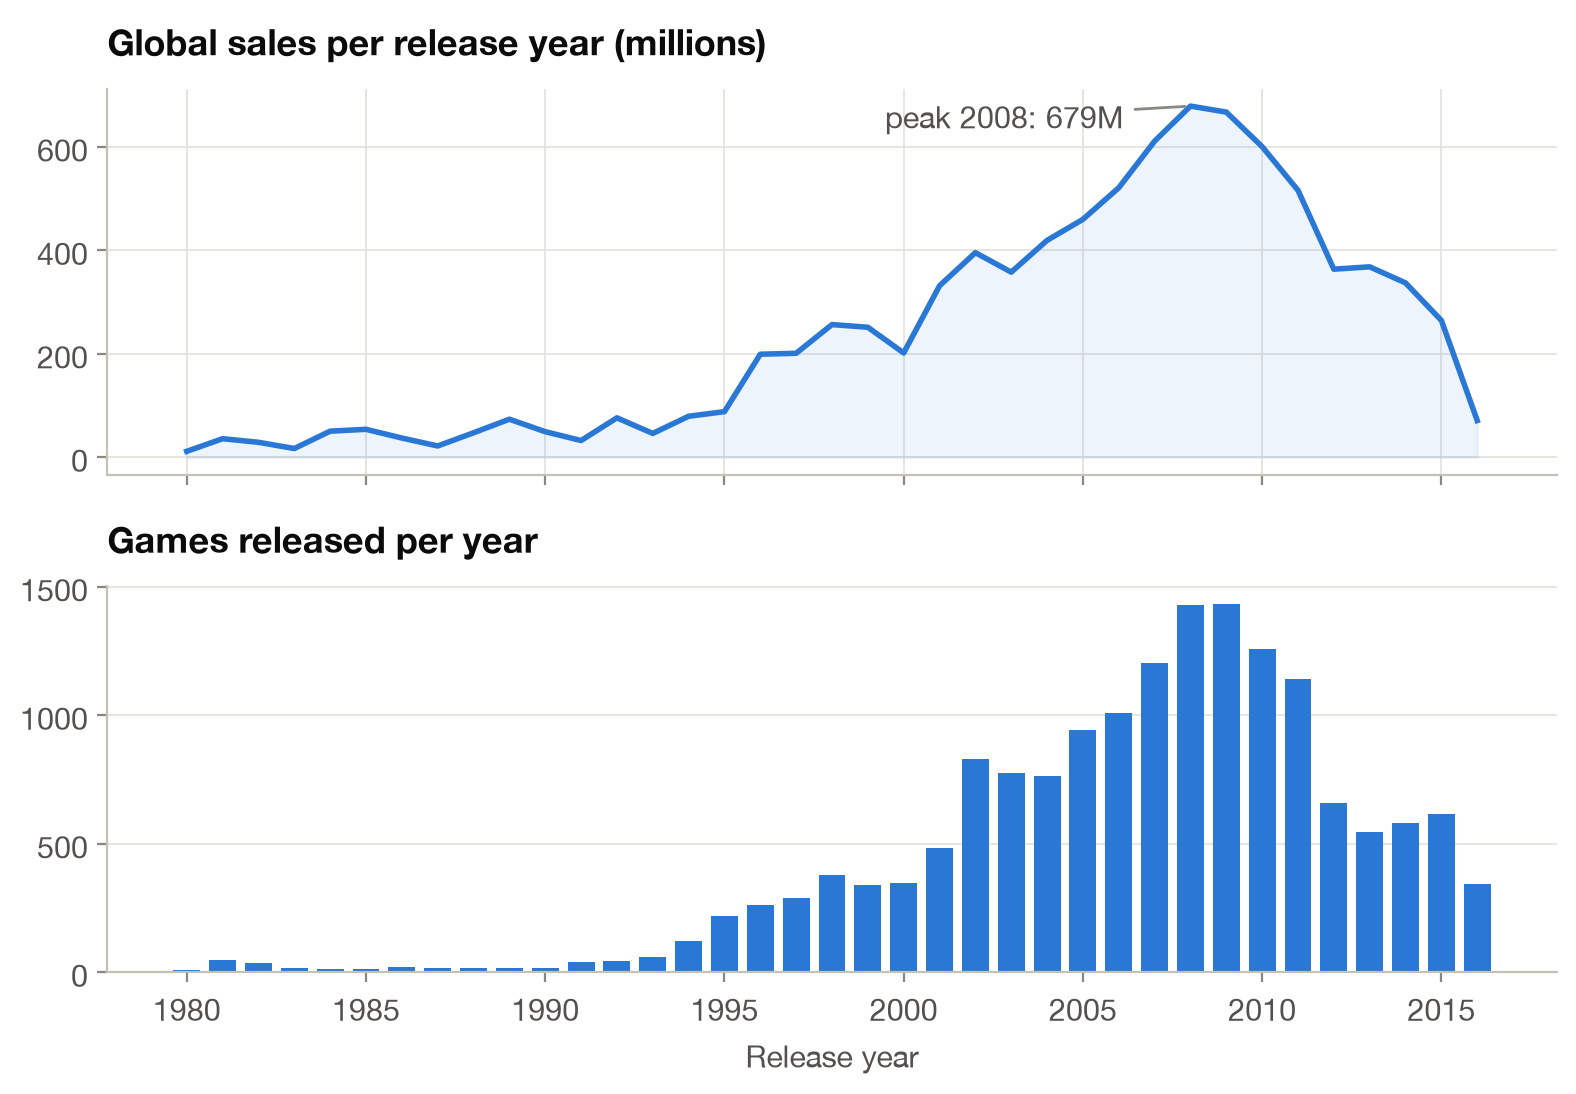
\includegraphics[width=0.49\linewidth]{vg_lifecycle.png}\hfill
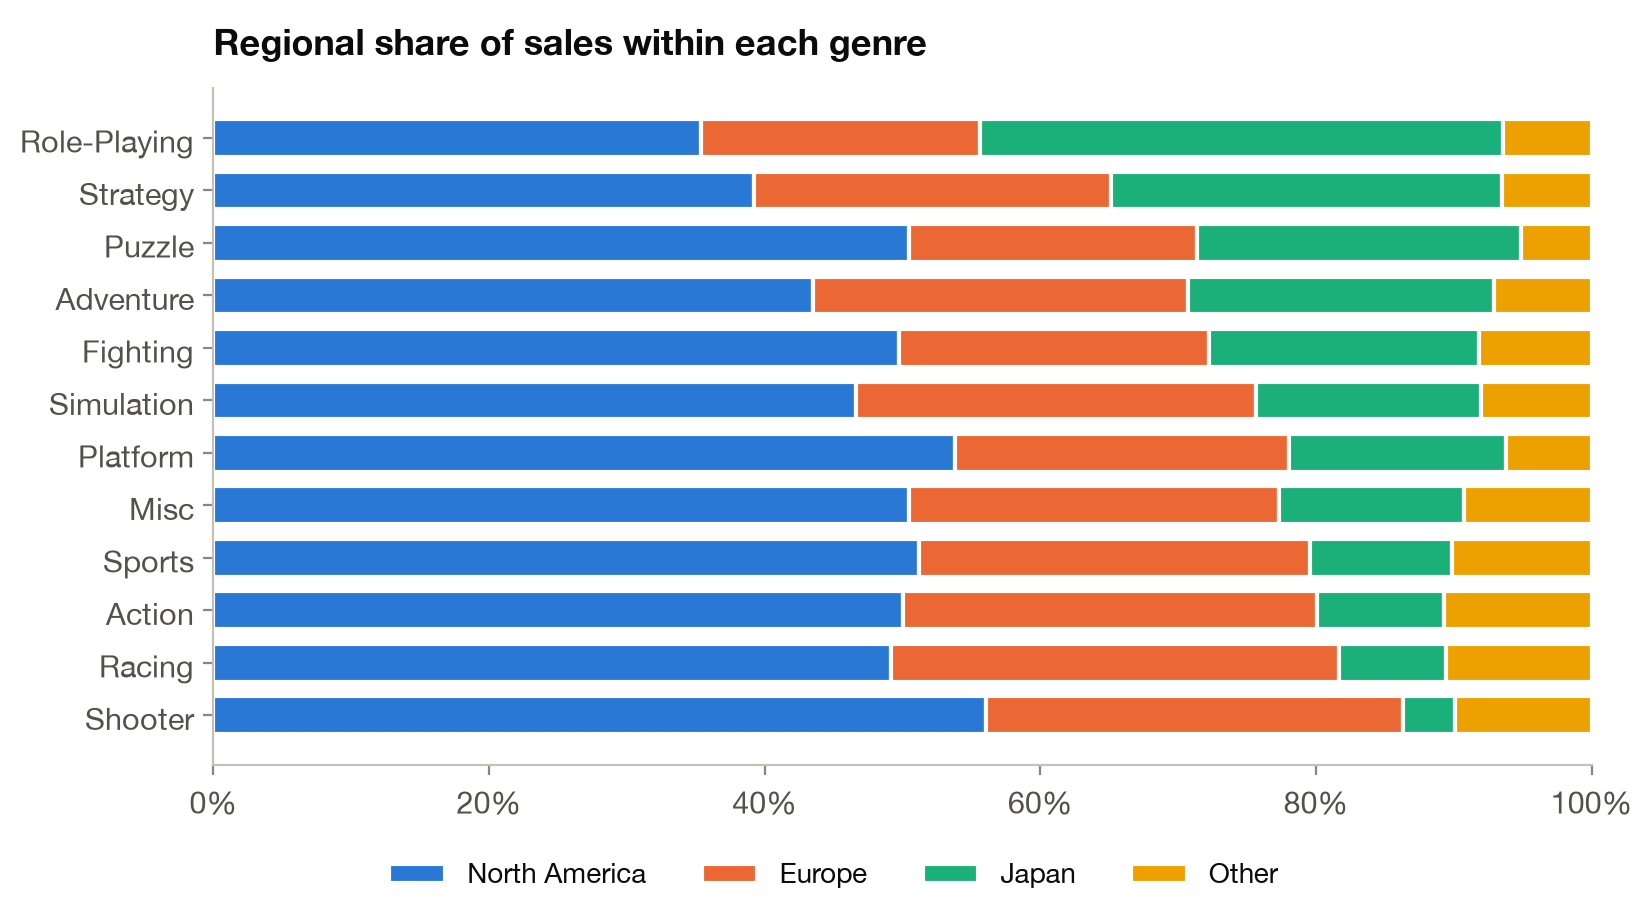
\includegraphics[width=0.49\linewidth]{vg_region_share_by_genre.png}
\caption{Video games: industry lifecycle 1980–2016 (left) and regional share of sales within each genre (right)}
\label{fig:vg}
\end{figure}
\textbf{Interpretation (Figure~\ref{fig:vg}).} The market is driven by hits. The median game sells 0.17 million copies,
while the top 1\% of games earn 21.1\% of all sales. Sales grew to a peak in 2008 (679 million units) and then declined;
the decline is partly real (the shift to digital and mobile) and partly an artefact of the data. North America accounts
for 49.1\% of sales, Europe 27.3\% and Japan 14.6\%. Japan behaves as a separate market: its sales correlate only 0.61
with global sales, against 0.94 for North America. Role-Playing is Japan's leading genre, and 38\% of all RPG sales are
Japanese.

\begin{figure}[H]
\centering
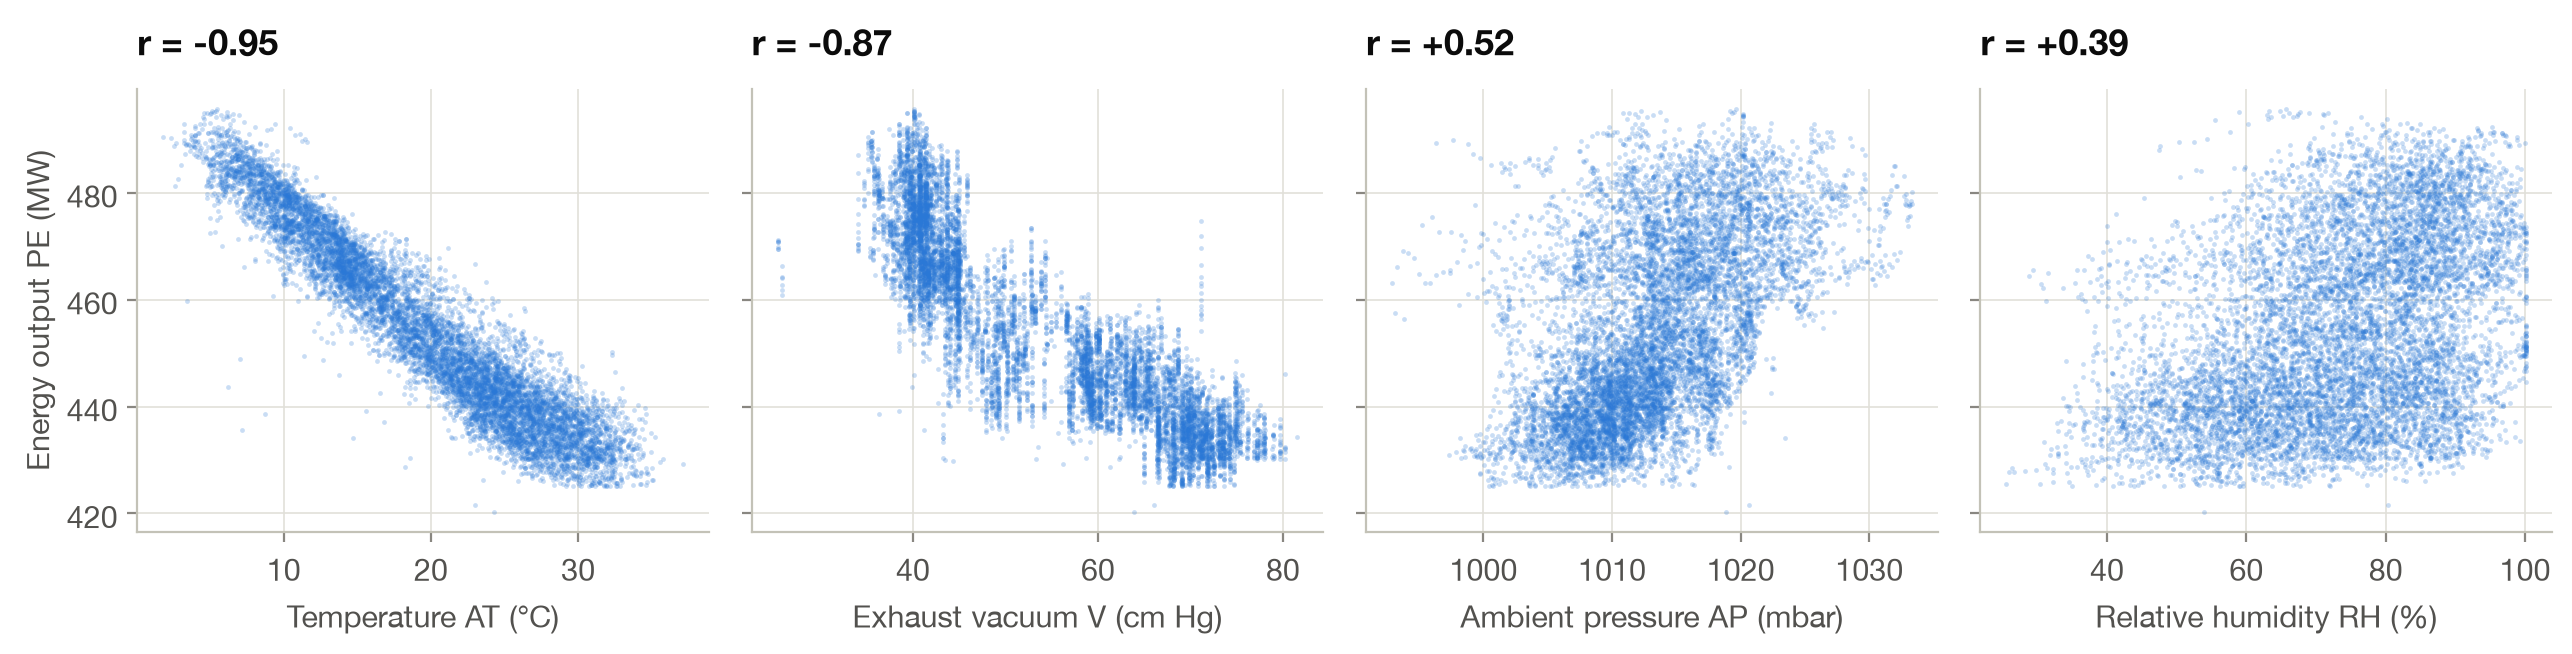
\includegraphics[width=\linewidth]{cc_feature_vs_target.png}
\caption{CCPP: each ambient feature against energy output PE, with Pearson correlation}
\label{fig:ccfeat}
\end{figure}
\textbf{Interpretation (Figure~\ref{fig:ccfeat}).} Temperature ($r=-0.95$) and exhaust vacuum ($r=-0.87$) are strong,
nearly linear negative drivers: hotter air is less dense, so the turbine produces less power. AT and V are correlated
with each other (variance inflation factors 6.0 and 3.9), which is moderate multicollinearity. The slight curvature of
the AT relationship suggests that non-linear models should help.

\begin{figure}[H]
\centering
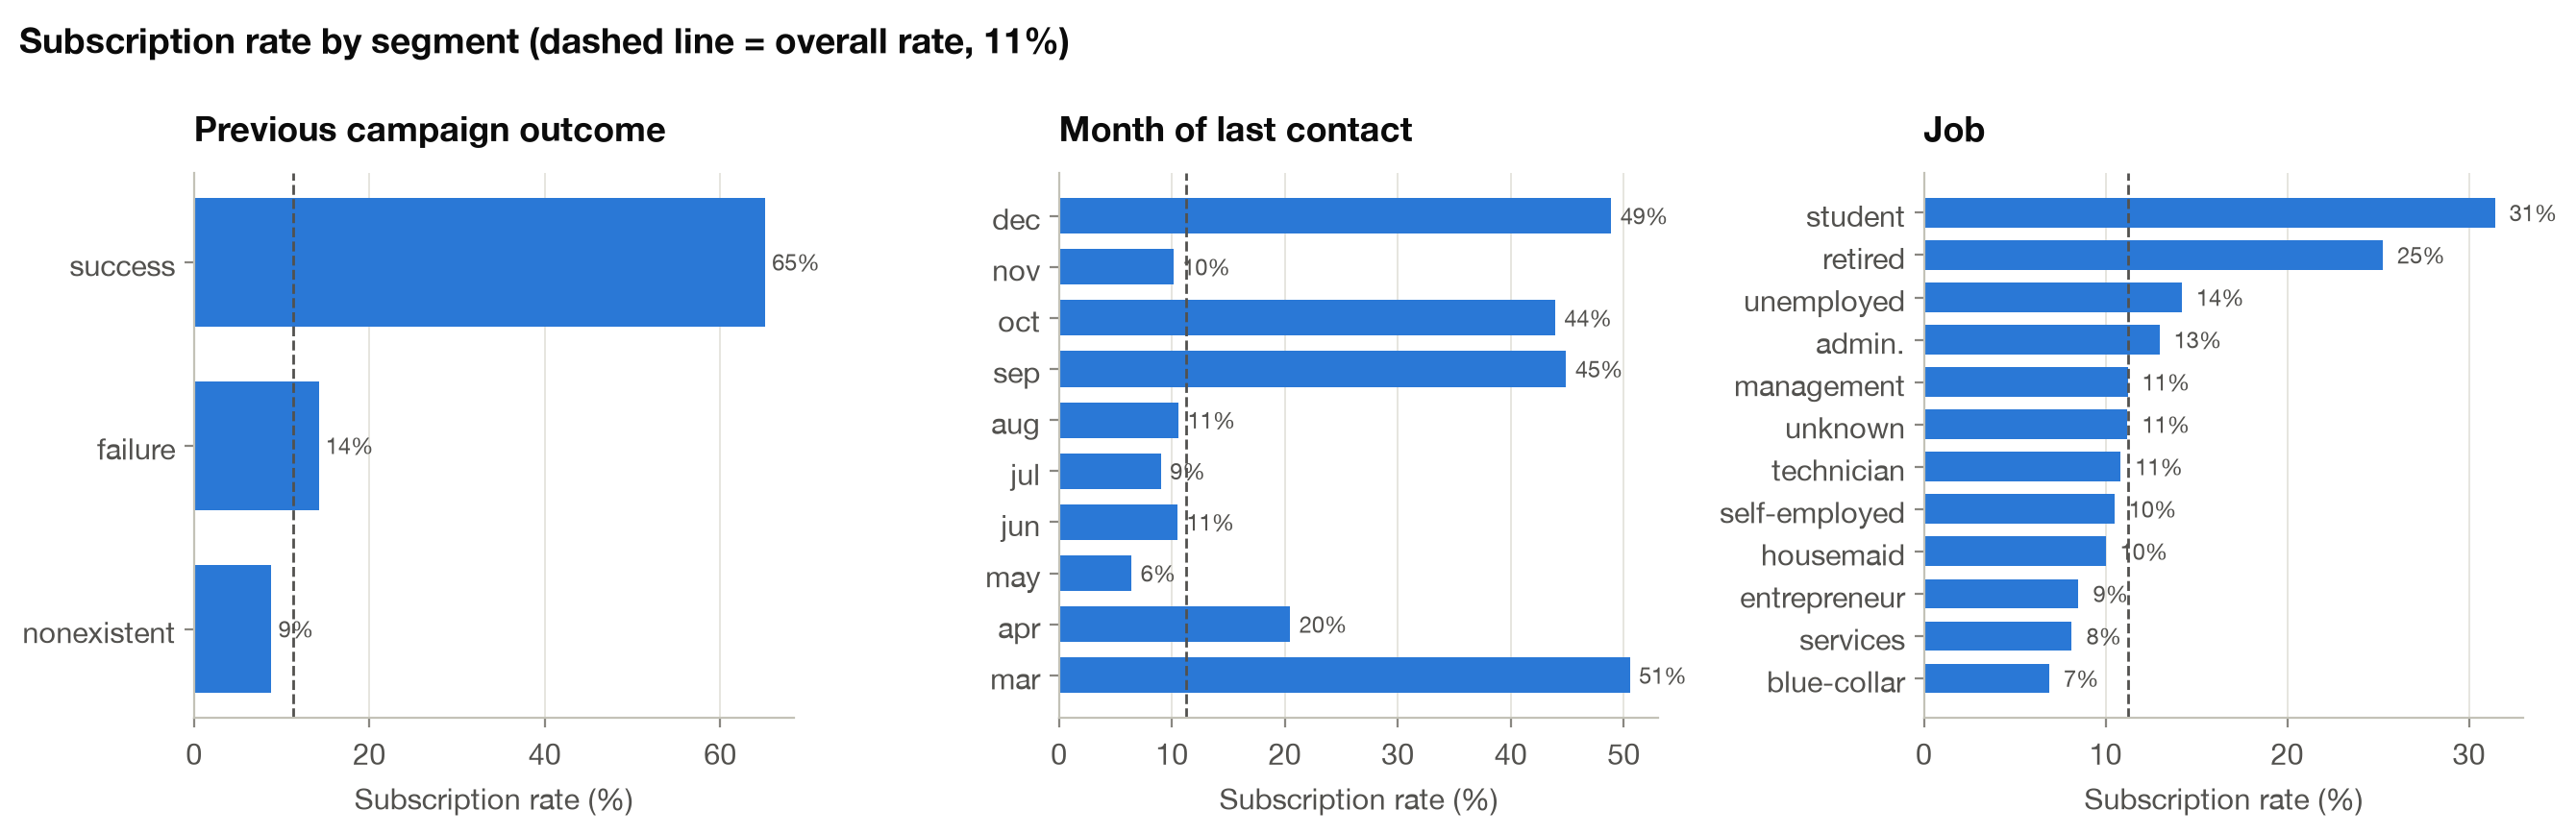
\includegraphics[width=\linewidth]{bk_rate_by_category.png}
\caption{Bank Marketing: subscription rate by previous-campaign outcome, month and job (dashed line = overall 11\%)}
\label{fig:bkrate}
\end{figure}
\textbf{Interpretation (Figure~\ref{fig:bkrate}).} Clients whose previous campaign succeeded subscribe 65\% of the
time. March, September, October and December convert at 44–51\% but are rarely used, while May has the most calls and
the lowest rate (6.4\%). Students (31\%) and retirees (25\%) are the most receptive groups.

\section{Proposed System Architecture / Workflow}
\begin{figure}[H]
\centering
\begin{tikzpicture}[node distance=0.45cm and 0.5cm, font=\small,
  box/.style={draw=navy, fill=lightblue, rounded corners=3pt, minimum height=1.1cm, text width=2.3cm, align=center},
  hl/.style={box, fill=lightorange, draw=accent}, arr/.style={-{Stealth[length=2.5mm]}, thick, navy}]
\node[box] (in) {Raw data\\(4 datasets)};
\node[box, right=of in] (aud) {Audit:\\types, duplicates, missing};
\node[box, right=of aud] (cl) {Cleaning \&\\feature engineering};
\node[box, right=of cl] (eda) {EDA \&\\insights (Unit 1)};
\node[box, below=1.1cm of cl] (split) {Train/test split\\(80/20, stratified)};
\node[box, left=of split] (pipe) {Pipeline: encode\\+ scale (train only)};
\node[hl, left=of pipe] (mod) {10+ models\\5-fold CV};
\node[box, right=of split] (tune) {Tuning \& threshold selection};
\node[hl, right=of tune] (eval) {Test-set evaluation\\\& interpretation};
\draw[arr] (in) -- (aud); \draw[arr] (aud) -- (cl); \draw[arr] (cl) -- (eda);
\draw[arr] (cl) -- (split); \draw[arr] (split) -- (pipe); \draw[arr] (pipe) -- (mod);
\draw[arr] (mod.south) |- ++(0,-0.5) -| (tune.south); \draw[arr] (tune) -- (eval);
\end{tikzpicture}
\caption{Workflow for Units 1 and 2}
\label{fig:wf12}
\end{figure}
Raw data is first audited (types, duplicates, missing values) and cleaned. The EDA branch (Unit 1) ends in insights.
The modelling branch (Unit 2) splits the data before any fitting. Encoding and scaling sit inside a pipeline so that
they are fitted on training folds only. More than ten models are compared with 5-fold cross-validation. The best family
is then tuned (GridSearchCV for regression; decision-threshold selection on out-of-fold predictions for classification),
and the held-out test set is used exactly once.

\section{Algorithm Theory and Mathematical Formulation}
\textbf{Linear regression} minimises the squared error; \textbf{Ridge} and \textbf{Lasso} add $L_2$ and $L_1$ penalties:
\begin{equation}
\hat{\boldsymbol\beta}=\arg\min_{\boldsymbol\beta}\ \sum_{i=1}^{n}\big(y_i-\mathbf{x}_i^\top\boldsymbol\beta\big)^2
+\lambda_2\lVert\boldsymbol\beta\rVert_2^2+\lambda_1\lVert\boldsymbol\beta\rVert_1 .
\end{equation}
\textbf{Logistic regression} models the probability of the positive class with the sigmoid and is fitted by minimising
the log-loss:
\begin{equation}
P(y=1\mid\mathbf{x})=\sigma(\mathbf{w}^\top\mathbf{x}+b)=\frac{1}{1+e^{-(\mathbf{w}^\top\mathbf{x}+b)}},\qquad
\mathcal{L}=-\sum_i\big[y_i\log p_i+(1-y_i)\log(1-p_i)\big].
\end{equation}
\textbf{Decision trees} split the data recursively to reduce impurity (Gini or variance). \textbf{Random Forest} averages
bootstrapped, decorrelated trees. \textbf{Gradient Boosting / XGBoost} \cite{friedman,xgboost} add trees sequentially, each one fitted to the
negative gradient of the loss (Chapter 4 covers these in depth). \textbf{KNN} predicts from the $k$ nearest neighbours,
and \textbf{SVR} fits an $\varepsilon$-insensitive tube in an RBF feature space. These methods follow \cite{esl,sklearn}. Class imbalance is handled by
class-weighting the loss (weight $\propto 1/\text{class frequency}$) or by SMOTE oversampling \cite{chawla} inside the CV folds.

\textbf{Evaluation metrics.}
\begin{equation}
\text{RMSE}=\sqrt{\tfrac{1}{n}\sum(y_i-\hat y_i)^2},\quad
\text{MAE}=\tfrac{1}{n}\sum|y_i-\hat y_i|,\quad
R^2=1-\frac{\sum(y_i-\hat y_i)^2}{\sum(y_i-\bar y)^2},
\end{equation}
\begin{equation}
\text{Precision}=\frac{TP}{TP+FP},\quad \text{Recall}=\frac{TP}{TP+FN},\quad
F_1=\frac{2\cdot\text{Precision}\cdot\text{Recall}}{\text{Precision}+\text{Recall}} .
\end{equation}
ROC-AUC is the probability that a randomly chosen positive is ranked above a randomly chosen negative. These methods are
appropriate because the CCPP relationships are smooth but slightly non-linear, which favours ensembles over linear
models. The bank data is imbalanced, which makes F1, recall and AUC the meaningful metrics and accuracy misleading.

\section{Results and Performance Evaluation}
\begin{table}[H]
\centering
\caption{CCPP regression: 5-fold CV and held-out test results (sorted by test RMSE)}
\label{tab:reg}
\begin{tabular}{@{}lcccc@{}}
\toprule
\textbf{Model} & \textbf{CV $R^2$} & \textbf{Test MAE (MW)} & \textbf{Test RMSE (MW)} & \textbf{Test $R^2$} \\
\midrule
\rowcolor{lightorange} XGBoost (tuned) & 0.9670 & 2.166 & \textbf{3.171} & \textbf{0.9658} \\
XGBoost & 0.9656 & 2.287 & 3.282 & 0.9633 \\
Gradient Boosting & 0.9623 & 2.441 & 3.404 & 0.9606 \\
Random Forest & 0.9598 & 2.409 & 3.434 & 0.9599 \\
KNN ($k=7$) & 0.9510 & 2.651 & 3.750 & 0.9521 \\
Decision Tree & 0.9417 & 2.933 & 4.075 & 0.9435 \\
SVR (RBF) & 0.9444 & 3.006 & 4.077 & 0.9434 \\
Polynomial (degree 3) & 0.9404 & 3.269 & 4.234 & 0.9390 \\
Lasso / Ridge & 0.9283 & 3.621 & 4.587 & 0.9284 \\
Linear Regression & 0.9283 & 3.621 & 4.587 & 0.9284 \\
\bottomrule
\end{tabular}
\end{table}
\begin{figure}[H]
\centering
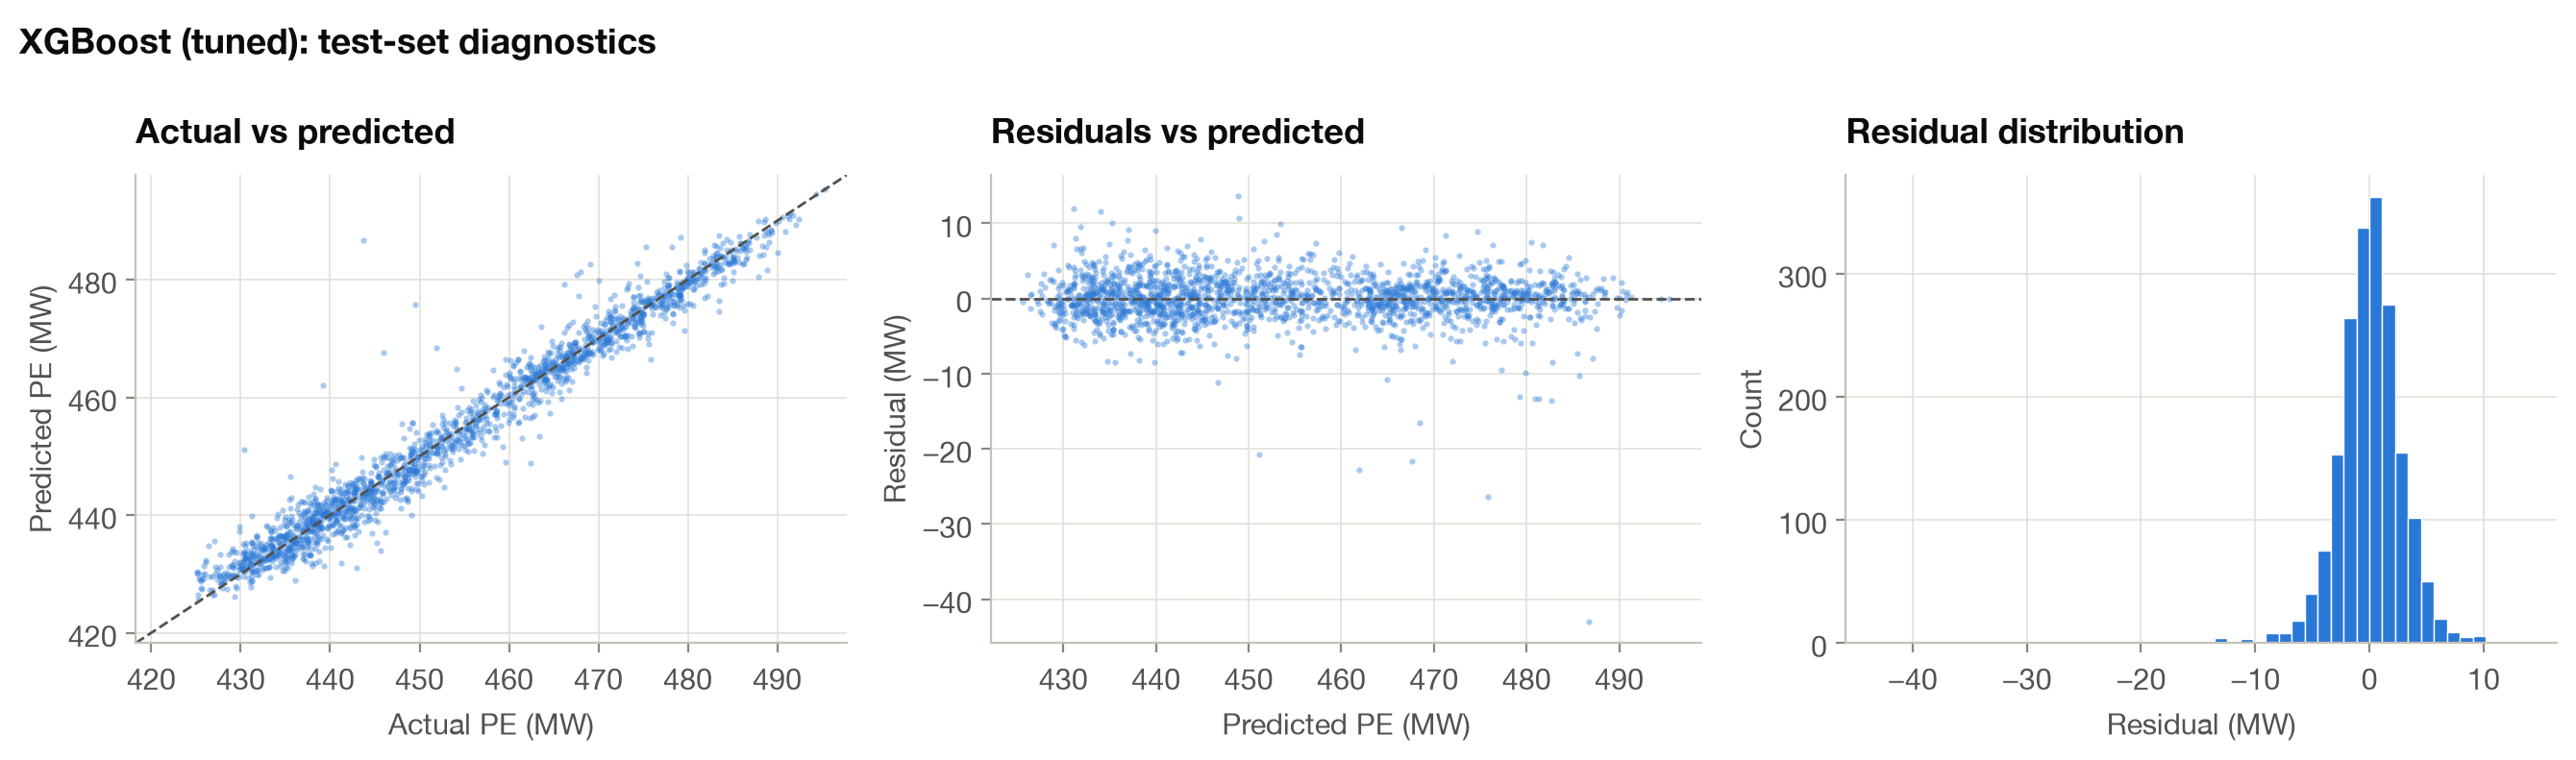
\includegraphics[width=\linewidth]{cc_best_diagnostics.png}
\caption{CCPP: tuned XGBoost test-set diagnostics (actual vs predicted, residuals, residual distribution)}
\label{fig:ccdiag}
\end{figure}
\textbf{Interpretation (Table~\ref{tab:reg}, Figure~\ref{fig:ccdiag}).} The tuned XGBoost model (1,200 trees, learning
rate 0.03, depth 7) has RMSE 3.17 MW and $R^2$ 0.966, which is \textbf{30.9\% lower error} than linear regression
(4.59 MW). 92.5\% of hourly predictions fall within $\pm$5 MW. Residuals are centred at zero with no pattern, so the
model shows no systematic bias. Ridge and Lasso match plain linear regression: with four features there is nothing to
regularise. CV $R^2$ agrees with test $R^2$ (standard deviation 0.003), so the ranking is stable. Permutation importance
confirms that temperature dominates.

\begin{table}[H]
\centering
\caption{Bank Marketing classification: held-out test results (sorted by F1)}
\label{tab:clf}
\begin{tabular}{@{}lccccc@{}}
\toprule
\textbf{Model} & \textbf{Accuracy} & \textbf{Recall} & \textbf{F1} & \textbf{ROC-AUC} & \textbf{PR-AUC} \\
\midrule
\rowcolor{lightorange} XGBoost (weighted, threshold 0.65) & 0.881 & 0.595 & \textbf{0.531} & \textbf{0.812} & 0.484 \\
Random Forest (balanced) & 0.873 & 0.617 & 0.523 & 0.807 & 0.484 \\
XGBoost (weighted, threshold 0.50) & 0.845 & 0.654 & 0.487 & 0.812 & 0.484 \\
Decision Tree (balanced) & 0.847 & 0.637 & 0.484 & 0.801 & 0.460 \\
Logistic Reg. (balanced) & 0.831 & 0.645 & 0.462 & 0.800 & 0.446 \\
Logistic Reg. + SMOTE & 0.822 & 0.654 & 0.453 & 0.799 & 0.445 \\
Naive Bayes & 0.808 & 0.624 & 0.423 & 0.776 & 0.359 \\
KNN ($k=15$) & 0.898 & 0.263 & 0.368 & 0.773 & 0.419 \\
Gradient Boosting & 0.899 & 0.233 & 0.342 & 0.811 & 0.480 \\
Logistic Regression & 0.898 & 0.212 & 0.320 & 0.801 & 0.453 \\
Baseline (always ``no'') & 0.887 & 0.000 & 0.000 & 0.500 & 0.113 \\
\bottomrule
\end{tabular}
\end{table}
\begin{figure}[H]
\centering
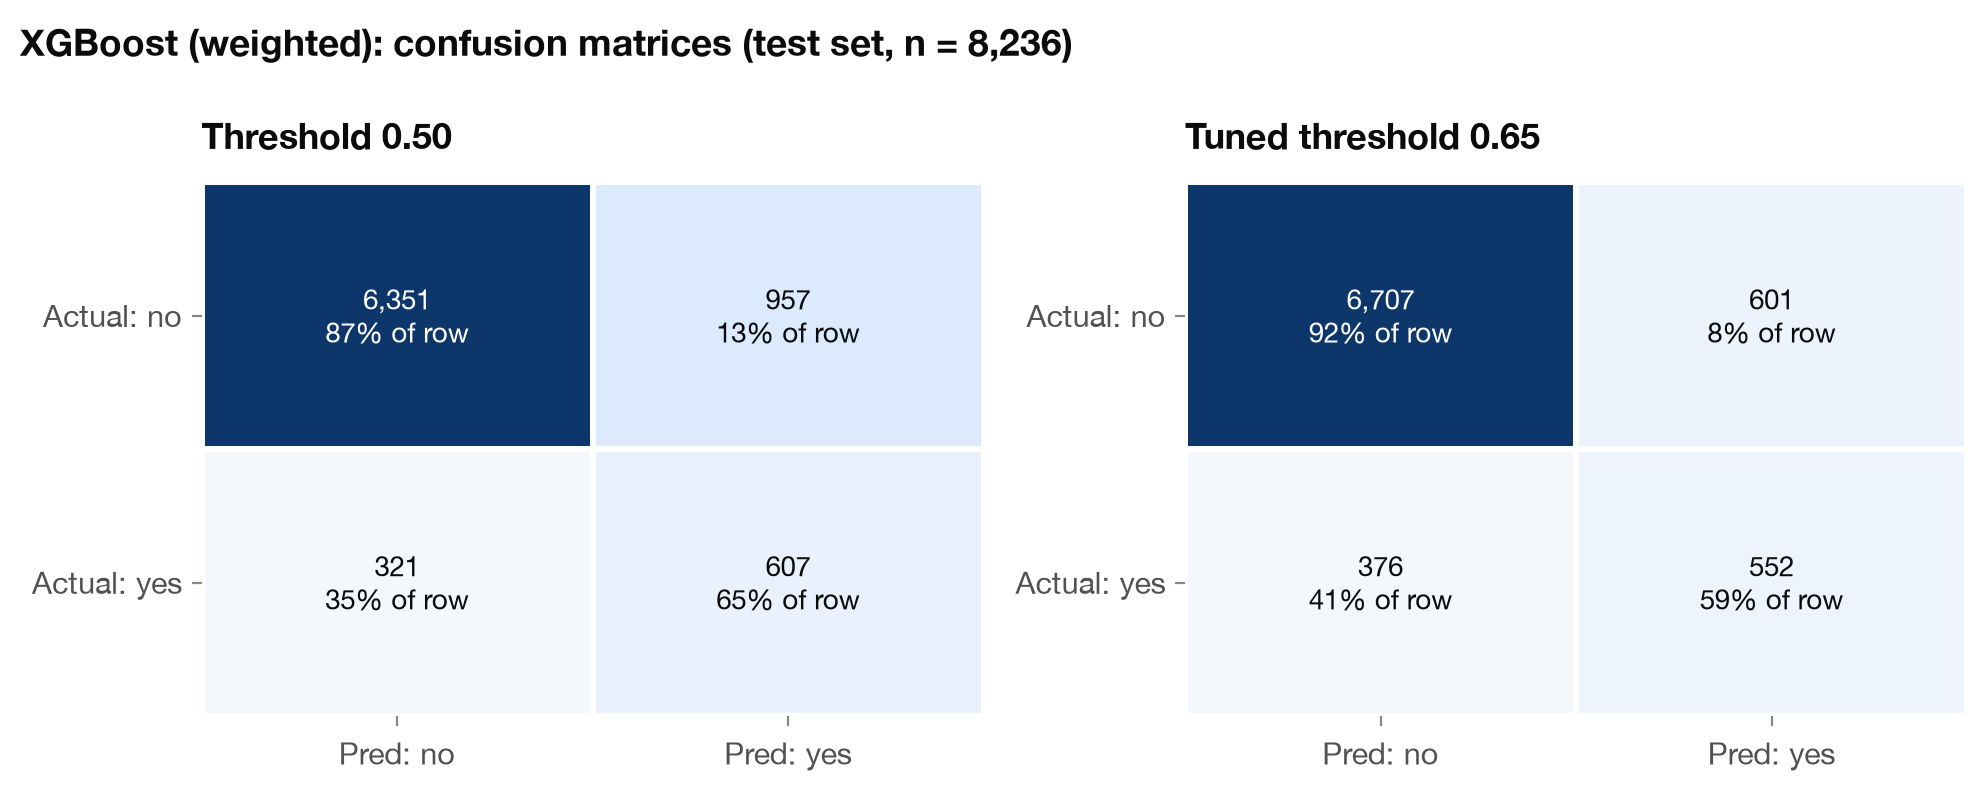
\includegraphics[width=0.52\linewidth]{bk_confusion.png}\hfill
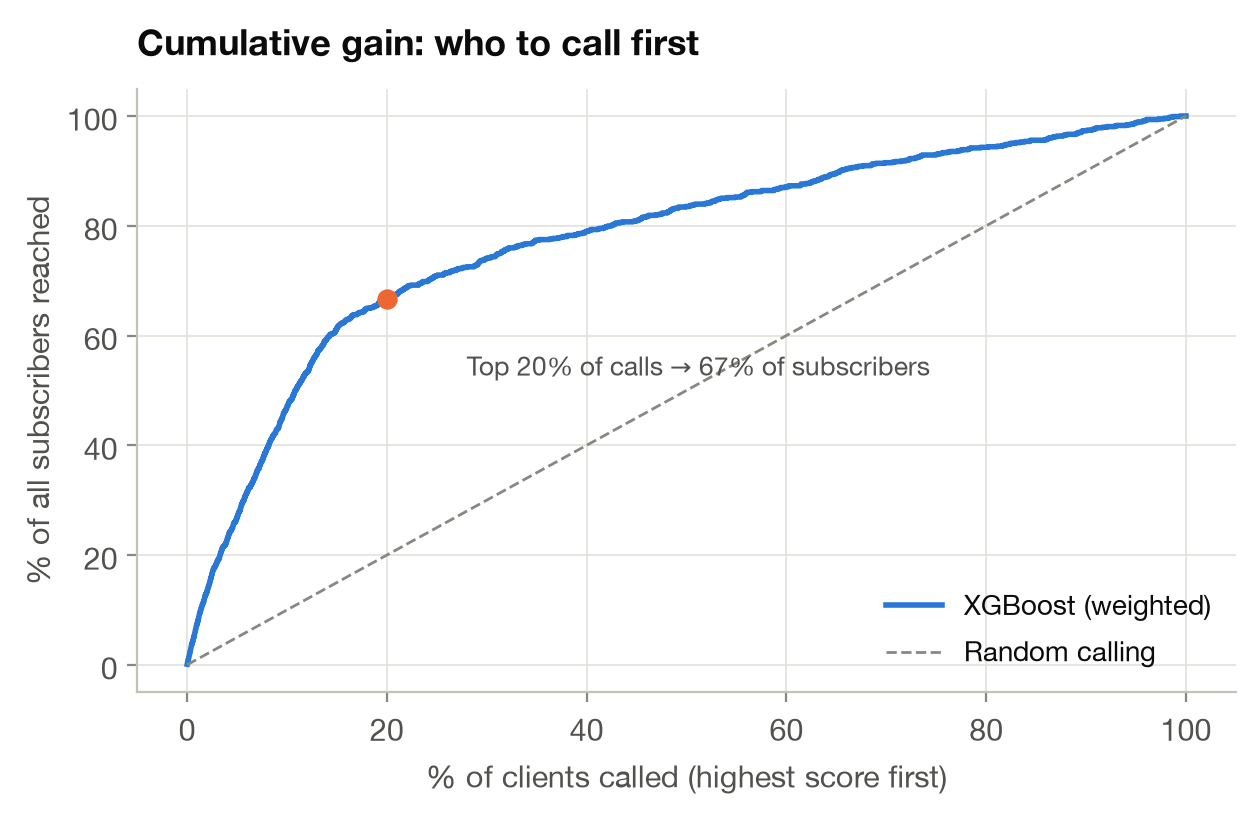
\includegraphics[width=0.46\linewidth]{bk_gain_curve.png}
\caption{Bank Marketing: confusion matrices at thresholds 0.50 and 0.65 (left), and cumulative gain (right)}
\label{fig:bk}
\end{figure}
\textbf{Interpretation (Table~\ref{tab:clf}, Figure~\ref{fig:bk}).} The \emph{accuracy trap} is clear: a model that
always predicts ``no'' is 88.7\% accurate but finds no subscribers, and plain logistic regression finds only 21\% of them.
Class weighting or SMOTE roughly triples recall at the same ROC-AUC. Class-weighted XGBoost with the F1-optimal threshold
(0.65, chosen on out-of-fold training predictions) is the best model (F1 0.531, ROC-AUC 0.812). Raising the threshold
from 0.50 to 0.65 cuts wasted calls from 957 to 601 (37\% fewer). Calling the top 20\% of clients ranked by the model
reaches 66.7\% of all subscribers, a \textbf{3.3$\times$ lift} over random calling.

\section{Discussion and Findings}
\begin{itemize}
\item \textbf{What worked:} tree ensembles (XGBoost, Random Forest) were the best models on both supervised tasks.
Pipelines prevented preprocessing leakage, and threshold tuning on out-of-fold predictions turned a good ranking model
into a useful decision rule.
\item \textbf{Challenges:} data quality dominated the EDA effort (text-encoded numbers, duplicates, informative
missingness). On the bank data, finding and removing the leaking \texttt{duration} feature was essential for a realistic
model. With it, published models report AUC above 0.9, which overstates what can be known before a call.
\item \textbf{Limitations:} the CCPP models used default settings except for XGBoost. The bank model's ROC-AUC ceiling of
about 0.81 reflects the limited information available before a call, and its macro-economic features are specific to
2008–2010.
\end{itemize}

\section{Chapter Conclusion}
PBL I delivered quantified market insights (Unit 1) and two well-validated supervised models (Unit 2): CCPP regression
with RMSE 3.17 MW ($R^2$ 0.966), and bank-marketing classification with F1 0.531, ROC-AUC 0.812 and a 3.3$\times$ lift.
These results set the baseline methodology used in the later chapters: audit-first cleaning, leakage-free pipelines,
cross-validated model comparison, metrics matched to the class balance, and a single use of the test set. They also
showed that gradient-boosted tree ensembles are strong on tabular data, a finding Chapter 4 tests directly.
